\chapter{Visualización de imágenes 3D}
\label{chap:visualizaImagenes}
En éste trabajo estamos interesados en visualizar campos escalares discretizados. Un campo escalar es un mapeo $f:\mathbb{R}^3 \rightarrow \mathbb{R}$ donde $f$ típicamente representa el valor de una cantidad física en el espacio. En la actualidad muchos dispositivos, por ejemplo los tomógrafos, son capaces de producir muestreos de estos campos. Dada la naturaleza electrónica de los dispositivos con los que medimos el campo escalar, en realidad se tiene una aproximación de $f$ que se obtiene, en general, muestreando de manera uniforme el espacio tridimensional. 

Para representar un punto en $\mathbb{R}^n$, alternativamente $\mathbb{Z}^n$, usaremos la representación $\textbf{p} \in \mathbb{R}^n$, alternativamente $\textbf{k} \in \mathbb{Z}^n$, y su $n$-tupla $\textbf{p} = \{ p_1, p_2,\ldots, p_n \}$ donde $p_i \in \mathbb{R}$, alternativamente $\textbf{k} = \{ k_1, k_2,\ldots, k_n \}$ donde $k_i \in \mathbb{Z}$. Debido a que usamos recursos finitos para llevar a cabo la discretización de $f$ solo usaremos un subconjunto $\Gamma \subset \mathbb{Z}^3$ definido de la siguiente manera:

\begin{equation}
\Gamma = \left\lbrace \textbf{k} | A_i \leq k_i \leq B_i \text{ para } 1 \leq i \leq 3 \text{ con } A_i < B_i \text{ y } A_i, B_i \in \mathbb{Z} \right\rbrace 
 \label{ec:escena}.
\end{equation}

Dado un punto $\textbf{k} \in \Gamma$ y un numero real positivo $\Delta$, definimos un vóxel cúbico como 
\begin{equation}
   \text{Vox} (\textbf{k}) = \left\lbrace \textbf{x} \in \mathbb{R}^3 | \Delta \left(  k_i - \dfrac{1}{2} \right) \leq x_i < \Delta \left(  k_i + \dfrac{1}{2} \right)  , \text{ para } 1 \leq i \leq 3 \right\rbrace 
  \label{ec:voxel},
\end{equation}al número $\Delta$ comúnmente se le conoce como distancia de muestreo\cite{edgarReconstruction}. El termino vóxel proviene del ingles \emph{volume element} y por lo tanto pueden existir vóxeles no cúbicos. Al mismo tiempo un punto $\textbf{k} \in \mathbb{Z}^2$ tiene asociado un píxel, proveniente del ingles \emph{picture element}. Debido a que en éste trabajo no utilizamos teselaciones no cúbicas, usaremos el término vóxel para referirnos a los vóxeles de \eqref{ec:voxel}.

  \begin{figure}[htp]
  \begin{center}
    \subfigure[$\tau = 61$]{\label{fig:mc61}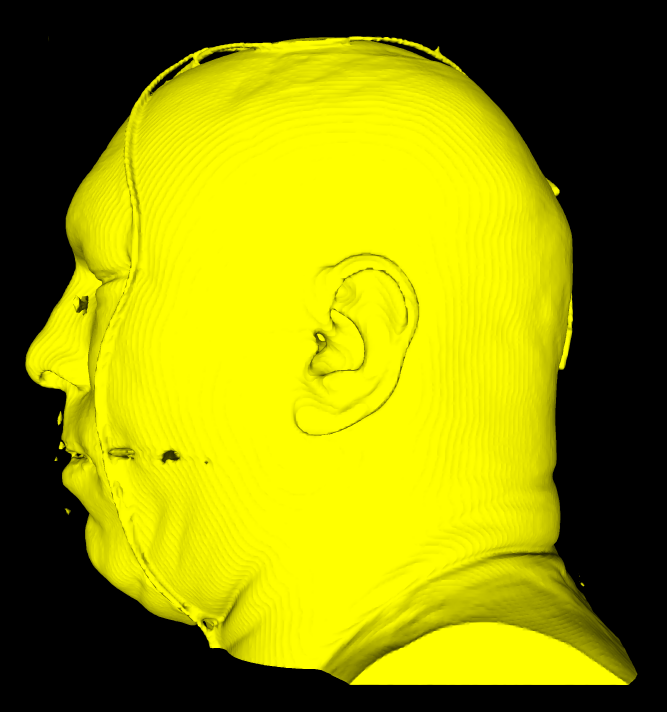
\includegraphics[scale=0.4]{img/cap01/mc61}}
    \subfigure[$\tau = 69$]{\label{fig:mc69}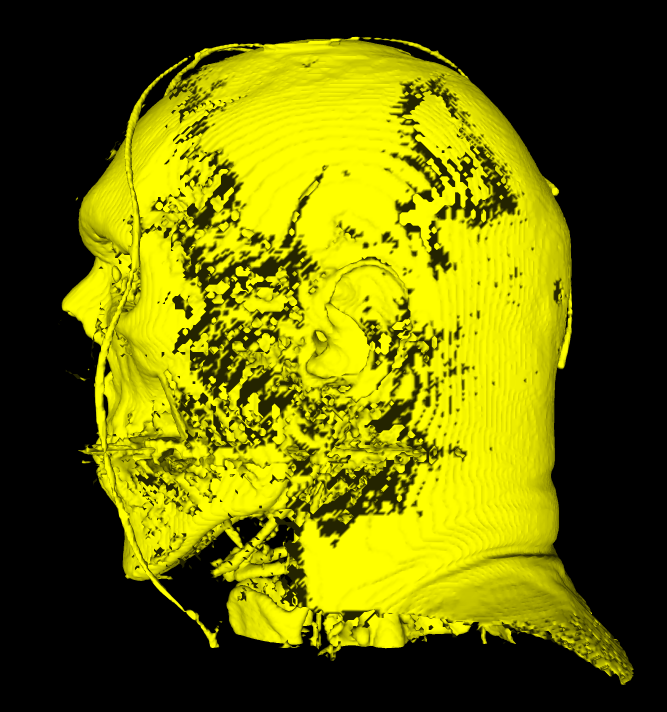
\includegraphics[scale=0.4]{img/cap01/mc69}} \\
    \subfigure[$\tau = 83$]{\label{fig:mc83}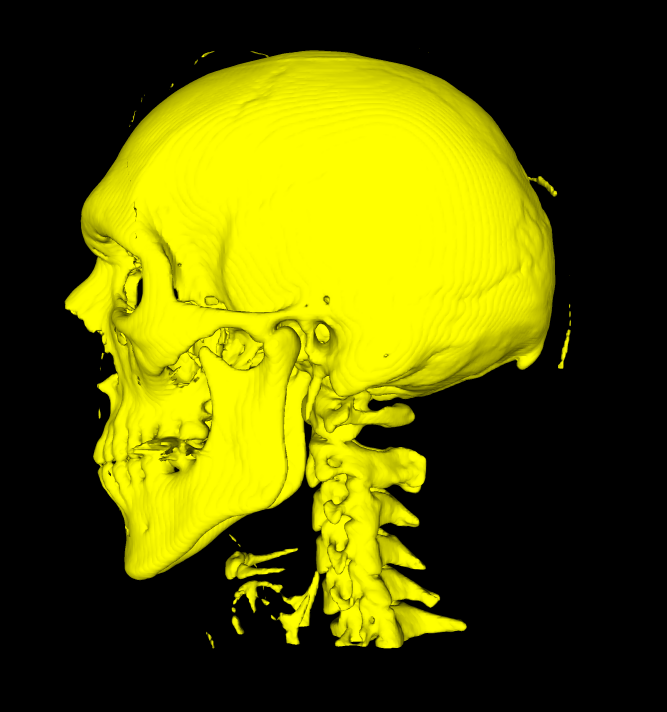
\includegraphics[scale=0.4]{img/cap01/mc83}}
    \subfigure[$\tau = 123$]{\label{fig:mc123}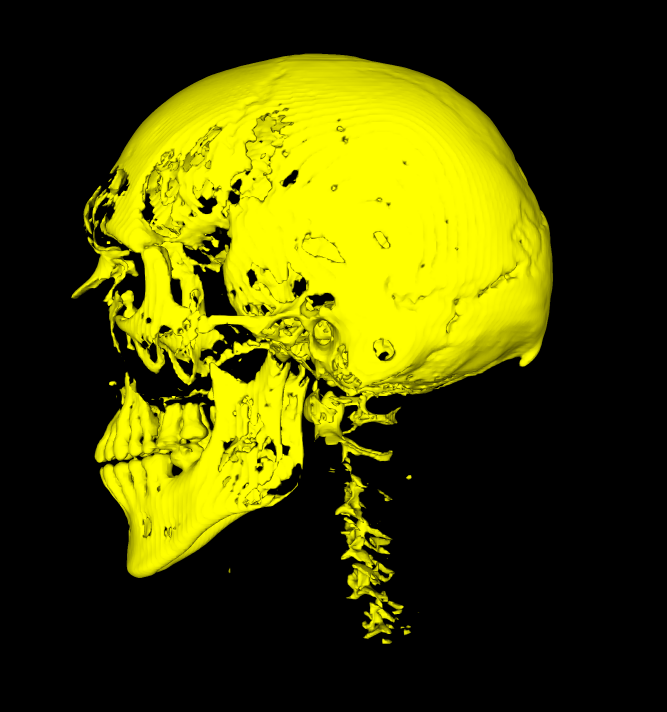
\includegraphics[scale=0.4]{img/cap01/mc123}}
  \end{center}
  \caption[Visualización por superficies de la imagen 3D con cuatro isovalores distintos]{Visualización por superficies de la imagen 3D con cuatro isovalores dentro del rango $[0,255]$ producida con el método de \emph{Marching Cubes}.}
  \label{fig:visIsoSurface}
  \end{figure}

\section{Adyacencias y caminos}

Antes de explicar como funcionan estos algoritmos necesitamos definir los conceptos de adyacencia y camino entre vóxeles

El concepto de \emph{adyacencia} entre dos vóxeles es una relación binaria simétrica sobre $\mathbb{Z}^3$. Se dice que dos vóxeles son vecinos cuando son adyacentes. Existen varias adyacencias, aquí solo vamos a utilizar dos de las más comunes.

El algoritmo se lista a continuación. Se asume que el volumen $v$, ha sido clasificado por algún criterio de segmentación para producir el volumen binarizado $B(v)$ y que de alguna manera se encontró un cara $\beta^0$ como semilla.

\begin{algorithm}[H]
\caption{Algoritmo de Artzy}
\label{algo:artzy}
\begin{algorithmic}[1]
\REQUIRE Un \emph{bel} inicial $\beta^0$ y el volumen binarizado $B(v)$.
\ENSURE Una lista $\mathcal{A}_{\tau}$ con todas las caras cuadradas que aproximan la superficie.
\STATE Colocar el \emph{bel} $\beta^0$ en la salida $\mathcal{A}_{\tau}$, agregar $\beta^0$ a $Q$ y poner dos copias de $\beta^0$ en $L$.
\WHILE{$Q \neq \emptyset$}
  \STATE Sacar una cara $\beta$ de $Q$
  \IF{$\beta^1 \in L$}
    \STATE Quitar a $\beta^1$ de $L$
  \ELSE
    \STATE Agregar a $\beta^1$ en $\mathcal{A}_{\tau}$, en $L$ y en $Q$
  \ENDIF
  \IF{$\beta^2 \in L$}
    \STATE Quitar a $\beta^2$ de $L$
  \ELSE
    \STATE Agregar a $\beta^2$ en $\mathcal{A}_{\tau}$, en $L$ y en $Q$
  \ENDIF
\ENDWHILE

\end{algorithmic}
\end{algorithm}
